
\chapter{Framework}

	El esquema común para clasificar perfiles teniendo en cuenta cierta característica consiste en: i) extraer rasgos textuales de los documentos del autor, en nuestro caso de los tweets; ii) construir una representación a nivel de tweet o del perfil y finalmente iii) entrenar un modelo de clasificación a partir de la representación elaborada. 
	\\
	Como se puede observar, existe un proceso de identificación de los features empleados para contrastar las características entre tipos de perfiles, haciendo que el desempeño del modelo de clasificación dependa directamente de la robustez de este paso. 
	\\
	Mediante la explotación de modelos de Aprendizaje Profundo, se pretende prescindir de rasgos extraídos manualmente que pudieran resultar ruidosos a los modelos clasificadores o dejar de capturar relaciones claves de la estructura semántica y/o sintáctica, como se expone en la Sección \ref{SOTA}.
	\\\\
	En este Capítulo se describe un \textit{framework} para llevar a cabo el perfilado de autores, basado en el empleo de rasgos abstractos obtenidos a partir de diferentes arquitecturas de DL y la combinación de las mismas.
	De manera general sus principales contribuciones son:

	\begin{itemize}
			\item Se propone un framework para el perfilado semi-supervisado de autores en redes sociales. El mismo lleva a cabo el aprendizaje de rasgos abstractos para la representación en un espacio latente de los tweets, y construye a partir de los mismos el modelado del perfil.
			
			\item Es presentada una combinación de rasgos de estilo a niveles de palabra, oración y otras estructuras gramaticales, para evaluar su influencia sobre la representación exclusiva mediante features extraidos por los modelos de DL. 
		
			\item  Se exponen distintas arquitecturas para modelar tweets y perfiles de usuarios dentro del mismo framework, que relacionen de manera diferente la información para realizar un estudio comparativo. Además se propone una clasificador para combinar estas modelaciones, basado en ML tradicional.	
	\end{itemize}

	\section{Rasgos a Nivel de Tweet}
	
	El análisis del historial de un perfil de usuario en redes sociales como Twitter, involucra una cantidad considerable de información textual, lo cual puede resultar desafiante para el entrenamiento de algunos modelos de DL, sobretodo debido a las relaciones a largo plazo que es necesario contemplar a la hora de clasificar un perfil o extraer sus rasgos.	
	Este fenómeno es independiente del nivel de supervisado con que se afronte la tarea y es conocido como \textit{information vanishing} \citep{hochreiter2001gradient}. Otros modelos son capaces de lidiar con este problema, sin embargo, están limitados por la complejidad temporal que poseen para analizar secuencias de texto, tal es el caso de la popular arquitectura \textit{transformer} donde cada capa de atención tiene  $O (n^2*d)$, con $n \text{ y } d$ la longitud de la secuencia y la dimensionalidad de sus elementos respectivamente. 
	Por estas razones separar la clasificación del perfil en distintos momentos analizando primero estructuras menos extensas (i.e., los tweets) y luego el perfil completo, constituye una alternativa en el empleo de DL.\\
	El enfoque empleado para este trabajo se apoya en una arquitectura modular para modelar la información textual primeramente a nivel de tweets  (\textit{Codificador}) y luego conformar una agregación de los mismos que sirva para describir y clasificar el perfil (\textit{Clasificador}).
	
	\subsection{CNN - LSTM}~\label{cnn-lstm}
	
	El modelo CNN - LSTM (\textit{Convolutional Neural Netowrk - Long Short Term Memory}) representado en la \figurename~\ref{cnn_lstm}, recibe como entrada un tweet, analizando la secuencia a nivel de palabra o a nivel de caracteres.
	\begin{figure}[!thb]
		\begin{center}
			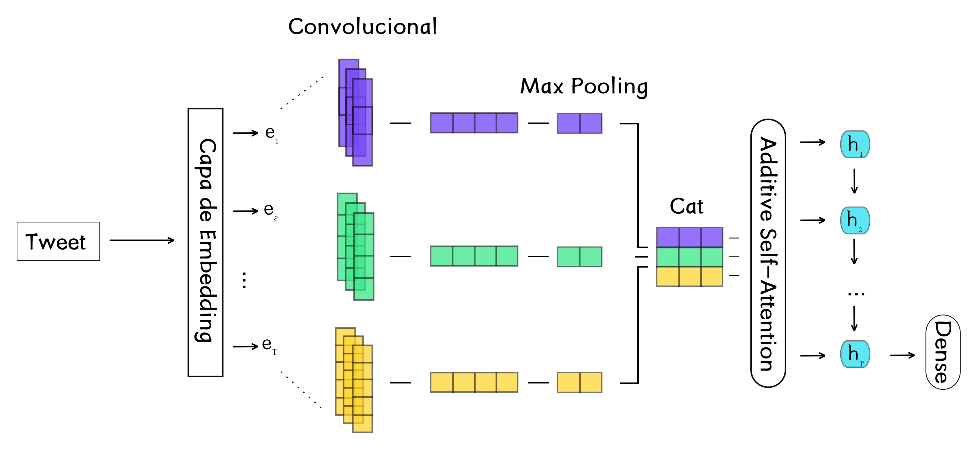
\includegraphics[]{images/cnn_lstm.eps}
		\end{center}	
		\caption[CNN - LSTM]{Arquitectura de Encoder CNN-LSTM}
		\label{cnn_lstm}
	\end{figure}
	\\
	Cada elemento de la secuencia es codificado por un \textit{embedding} de palabras o caracteres según sea el caso del análisis. En el primero, el modelo emplea un embedding preentrenado con representaciones fijas aprendidas mediante \textit{Word2Vec} de Google \citep{DBLP:conf/nips/MikolovSCCD13}. Mientras que a nivel de caracteres estas representaciones son inicializadas de manera aleatoria y aprendidas durante el proceso de entrenamiento del modelo completo.
	\\
	Como salida de esta capa de embedding obtenemos una matriz de valores reales $E \in \Re^{l\times d}$, con $l$ la longitud de la secuencia y  $d$ la dimensionalidad de la representación vectorial de sus elementos. Luego es aplicada la operación convolución en $1D$ mediante una capa de red convolucional, simulando el análisis de \textit{n-gramas} de palabras o caracteres sobre la representación del embedding que en este punto ya ha capturado ciertas relaciones de contexto entre los elementos del texto.
	\\
	Esta capa convolucional estará compuesta por filtros de distintos tamaños de ventana (3, 4, 5) inspirada en las Redes de Entradas (\textit{Inception Neural Networks}) \citep{szegedy2014going} para capturar relaciones espaciales dentro de la secuencia a corto plazo. Para cada tamaño de ventada (i.e., 3, 4 y 5) se emplean además 32 filtros que aprenden estas relaciones de manera independiente. 
	\\
	Una vez efectuada la convolución, sea $k$ el tamaño de la ventana, la longitud de la secuencia queda reducida a $l-k + 1$, luego para cada $k$ es aplicada la operación de \textit{max-pooling}, mediante la cual el modelo aprenderá a preservar solamente la información más relevante dentro de un \textit{n-grama}. El pooling se realiza de manera que en el paso $i-esimo$ la ventana no contempla los datos analizados en el paso $(i-1) -esimo$ por lo que el salto es equivalente al tamaño de la ventana, reduciendo nuevamente la secuencia a $\lceil\frac{l - k + 1}{k}\rceil$.
	\\
	La concatenación resultante de la\textit{ Inception Network} es considerada como una nueva secuencia de mapeo de rasgos, sin embargo, cada uno sus elementos se relacionan entre si aportando información relevante o no sobre la tarea a la cual responde el entrenamiento del modelo. Esta secuencia es procesada por una capa de \textit{self-attention} \textcolor{darkblue}{(Sección~\ref{atencion})} para ponderar los features teniendo en cuenta su nivel de importancia en vez de hacer a la red neuronal prestar atención de la misma forma a todos los elementos.
	\\
	Una vez combinada la información a través del mecanismo de atención, la secuencia es explorada y condensada por una LSTM, en la cual el fenómeno de \textit{information vanishing} estará inhibido gracias al mecanismo de atención. De la salida de la LSTM es preservado solamente el último estado oculto en el cual quedan capturadas relaciones a largo plazo en del estilo del autor y contenido del texto, finalmente es transformado a un elemento de un espacio latente por medio de una capa densa. Esta transformación constituye la representación del tweet con el que fue alimentado el modelo. 
	
	\subsection{Codificación basada en Transformers}\label{ref_trans}
	
	Teniendo en cuenta que al analizar individualmente los tweets la cantidad de información a procesar es reducida considerablemente y la capacidad de ``comprensión'' del lenguaje que han demostrado los modelos basados en arquitecturas Transformers (TM), se propone el empleo de modelos pre-entrenados para modelar representaciones abstractas de los tweets. Para ello primeramente se realiza un proceso de refinado (\textit{fine-tuning}) empleando la librería HuggingFace Transformers\footnote{\url{https://huggingface.co/transformers}} con datos que respondan a la tarea sobre la cual se llevará a cabo el perfilado. 
	\\\\
	En el proceso de \textit{fine-tuning} se añade una capa intermedia que recibe los vectores de la secuancia de salida del TM. En esta secuencia de features, se preserva solamente el vector asociado al \textit{token} [CLS]. Luego esta capa intermedia se apila una capa de salida encargada de realizar las predicciones para la tarea sobre la cual  se refina el modelo.
	\\
	Para cada uno de los bloques codificadores del encoder del Transformer es empleado un coeficiente de aprendizaje \textit{learning rate} distinto teniendo en cuenta un refinado gradual-discriminativo de cada bloque, incrementándolo a medida que la red se vuelve mas profunda. Esto es, $\alpha_i = \lambda_i \alpha_0 \text{ y } \lambda_i = \lambda_{i-1} + 0\text{.}1$, donde $\alpha_i$ representa el \textit{learning rate} del $i-esima$ bloque y $\lambda_i$ es un multiplicador para determinar $\alpha_i$ a partir de $\alpha_0$. Empleando este \textit{learning rate} dinámico se preserva la mayor cantidad de informacion aprendida durante el proceso de pre-entrenado el las capas más superficiales, encargadas de capturar rasgos generales, y se sesga el aprendizaje de las capas más profundas hacia la tarea específica abordada en el perfilado.
	\section{Modelado  y Clasificación del Perfil}
	
	Una vez sintetizada la información abstracta de los tweets, es importante la forma en la que se relaciona cada uno para clasificar el perfil, para ello se propone asumir el conjunto de los tweets como i) una secuencia y ii) una estructura basada en grafos.
	
	\subsection{Modelado Secuencial. Att-LSTM}\label{att-lstm}
	
	Aun cuando no existe necesariamente una relación temporal que exprese particularidades del estilo de escritura del perfil, es posible agregar la información de los tweets mediante una LSTM. Para ello, en el proceso de entrenamiento se construye una secuencia con los tweets, y en cada ciclo de entrenamiento (i.e., \textit{epoch}) de la red neuronal, esta secuencia es permutada aleatoriamente para evitar que el modelo capture erroneamente cualquier relación temporal. La \figurename~\ref{att_lstm} muestra la arquitectura general del modelo \textbf{Att-LSTM} (\textit{Attention- Long Short Term Memory}) empleada para modelar como secuencia el perfil y clasificarlo.
	
	\begin{figure}[!thb]
		\begin{center}
			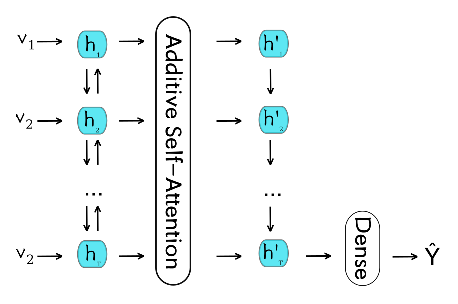
\includegraphics[]{images/att_lstm.eps}
		\end{center}	
		\caption[Att - LSTM]{Modelado y Clasificación del Perfil. Att-LSTM}
		\label{att_lstm}
	\end{figure}
	
	El modelo recibe una secuencia donde cada elemento corresponde a los rasgos extraídos para un tweet del perfil, esta secuencia es enviada a una LSTM Bidireccional (Bi-LSTM) \citep{DBLP:journals/tsp/SchusterP97}, la cual consiste en una célula de LSTM de 64 unidades que calcula para cada elemento dos estados ocultos concatenados, uno de ellos correspondiente a un recorrido de izquierda a derecha y el otro en sentido contrario.
	\\
	La Bi-LSTM no detecta solamente relaciones de un elemento con los previos en la secuencia sino que también lo relaciona con los que aparecen posteriormente, de esta forma se capturan las relaciones independientes de la posición de cada tweet dentro de la secuencia.
	\\ 
	La salida de la Bi-LSTM es enviada a una capa de \textit{self-attention} para emplear la misma estrategia propuesta en la \textcolor{darkblue}{Sección~\ref{cnn-lstm}} y luego a una capa de LSTM simple, donde nuevamente se preserva el último estado oculto y se condensa su información en una capa densa. Este modelado el perfil, finalmente es enviado otra capa densa encargada de clasificar el perfil según la tarea para la que se entrene el modelo.
	
	\subsection{Modelado basado en Grafo. SGN}\label{sgn}
	
	Dentro de las redes sociales en muchas ocasiones la información contextual es compartida de manera dispersa, e.g., el contenido de una idea relacionada con la difusión de odio puede ser construido relacionando la información de diferentes posts no necesariamente subidos de manera secuencial. Algunos trabajos han mostrado la importancia del contenido en tareas de AP \citep{OrtegaMendoza2018EmphasizingPI}, afirmando que rasgos basados en contenido a veces son más discriminativos que rasgos de estilo \citep{reddy2016survey}. Todo esto sugiere la idea de emplear una modelación no euclidiana del conjunto de tweets codificados y compartir la información de un tweets a los otros mientras que su información individual es transformada para expresar como este pertenece a su contexto.
	Las Redes Neuronales basadas en Grafo están especializadas en aprender patrones de este tipo de representaciones no estructuradas.
	\\
	El perfil es por tanto modelado con una representación basada en grafos, donde cada nodo es un tweet y cada uno de ellos esta conectado con todos los otros. Luego, este grafo es procesado por una Red Neuronal Convolucional Espectral en Grafos (\textit{Spectral Graph Convolutional Neural Network SGN}).
	\\
	El hecho de que cada nodo en el grafo modelado este conectado a todos los otros, hace que luego de un ciclo de paso de mensajes, un nodo individual, tenga conocimiento sobre cada nodo en el grafo, empleando el operador convolucional propuesto en \citep{kipf2017semisupervised} definido como:
	
	\begin{align}\label{matrix-wise}
		X' = ReLU(\hat{D}^{-\frac{1}{2}}\hat{A}\hat{D}^{-\frac{1}{2}}X\Theta)
	\end{align}
	
	Donde $X$ es la matris de representaciones vectoriales de los nodos, $\hat{A} = A + I$ es la matriz de adyacencia $A$ agregada a la matriz identidad $I$ lo que implica que autoconexiones para cada nodo son introducidas a la representación para que en el proceso de agregación se preserve su información original. La matriz $D$ es una matriz diagonal que contiene el grado del nodo $i-esimo$, i.e., $D_{ii} = |V|$ con $V$ el conjunto de los vértices. Finalmente, $\Theta$ es la matriz de parámetros de aprendizaje para determinar la codificación de cada nodo con sus rasgos que junto a la Matriz Laplaciana Normalizada expresan el nivel de variación entre los rasgos de los nodos dentro del grafo.
	\\
	Dada la formulación matricial de esta operación, a nivel de nodo esta queda definida como: 
	
	 \begin{align}\label{node-wise}
	 	x_i' = ReLU\left( \Theta \sum_{j \in \mathcal{N}(i) \cup \{i\}} \frac{1}{ 	\sqrt{ \hat{d_j} \hat{d_i} } }x_j \right)
	 \end{align}
	 \\
	 Aquí, $x_i$ representa la codificación del nodo $i-esimo$, $d_i$ el grado del mismo y $\mathcal{N}(i)$ su conjunto de nodos vecinos.
	 \\ 
	 Como es posible observar en \ref{node-wise} y \ref{matrix-wise}, en este esquema convolucional la información es compartida simplemente mediante una suma normalizada antes de calcular la nueva codificación $x_i'$ mediante $\Theta$.
	 \\
	 En la red convolucional propuesta este proceso de paso de mensaje y actualización es repetido a través de dos capas convolucionales. Luego, la información de los nodos es combinada a través de una capa de $mean-pool$ para alimentar una capa densa que sintetice la información. La salida de esta última capa es considerada como la modelación del perfil y es enviada a otra capa densa para realizar la clasificación.
	 
	 \section{Clasificación basada en ML. Deep Impostor }
	 
	 Un hecho interesante de sobre los modelos de DL es que a pesar de ser potentes a la hora de detectar rasgos abstractos que permitan particionar el espacio de representaciones en diferentes clases, cuando la cantidad de datos disponibles para el entrenamiento no es suficiente, su desempeño se ve afectado. Por esto se propone emplear las modelaciones  en un espacio latente de los perfiles descritas en la Sección~\ref{att-lstm} y Sección~\ref{sgn} con el Método Profundo de los Impostores \textit{(Deep Impostor Method DIM)} basado en el Método de los Impostores \citep{seidman2013authorship}, para realizar un estudio comparativo del desempeño en la clasificación binaria.
	 \\\\
	 Como en el método original, para realizar una predicción sobre un objeto desconocido (en este caso un perfil de autor) es definido previamente un conjunto $H$ y $K$ de ejemplos positivos y negativos respectivamente y el objeto desconocido $u$.
	 \\
	 De $H$ es muestreado de manera uniforme un subconjunto $\bar{H}$ como prototipos de la clase positiva y es analizado para cada $\bar{H}_i$ si $u$ es mas similar a este prototipo que a los elementos de un conjunto $\bar{K}_i$, i.e., $\mathcal{F}(u, \bar{H}_i) > \mathcal{F}(u, \bar{K}_{ij})$ donde $\mathcal{F}$ es una función de similitud; en este caso coseno. Luego de esto, se dice que $u$ teniendo en cuenta $\bar{H}_i$ es un candidato a pertenecer a una clase positiva según un voto por mayoría, esto es:
	 
	\begin{equation*}
	 	P_i(u,  \bar{H}_i) = 
	 	\begin{cases}
	 		1 & \text{if}~~ \sum\limits_{j}^{|\bar{K}_{i}|}[\mathcal{F}(u, \bar{H}_i) > \mathcal{F}(u, \bar{K}_{ij})] > \frac{|\bar{K}_{i}|}{2}\\
	 		0 & e.c.o.c
	 	\end{cases}
	 \end{equation*}	  
	 \\
	 Como los rasgos de los objetos serán aprendidos por medio de los modelos de DL descritos, es obviado el procedimiento de selección de rasgos expuesta en el método original, debido a que remover de manera indiscriminada alguno de ellos puede resultar en la destrucción de relaciones de similitud interclase o intraclase.
	 \\
	 Luego de definido cada $P_i$, un perfil $u$ es clasificado según la regla:
	 
	\begin{equation*}
	 	\hat{y}(u)  = 
	 	\begin{cases}
	 		1 & \text{if}~~ \sum\limits_{i}^{|\bar{H}|} P_i(u, \bar{H}_i) > \frac{|\bar{H}|}{2}\\
	 		0 & \text{otherwise}
	 	\end{cases}
	 \end{equation*}	
	 
	 
	 \section{Rasgos Manuales de Estilo}~\label{syle_feat}
	 
	 Para la representación del perfil es analizado un conjunto de 177 rasgos que capturen características relevantes del estilo de escritura. Los rasgos son estructurados en seis subconjuntos considerando diferentes capas textuales. Las capas son: booleanas; caracteres; oraciones; párrafo; sintáctica y de documento.
	 \\
	 Ejemplos de los elementos de estas capas son:	 \\
	 \begin{enumerate}
	 	\item Capa booleana: Usos de la misma palabra para terminar una oración y comenzar la siguiente.
	 	\item Capa de caracter: Media de la longitud de las palabras.
	 	\item Capa de oración: Media de la cantidad de palabras. Media de la cantidad de preposiciones distintas.
	 	\item Capa de párrafo: Media de la cantidad de oraciones. Media de la cantidad de palabras.
	 	\item Capa sintáctica: Proporción de sustantivos y adjetivos.
	 	\item Capa de documento: Media de la longitud de las oraciones.
	 \end{enumerate}
	 Esta representación es completamente independiente del genero textual e involucra valores con distintas estructuras de datos como se muestra en la \figurename~\ref{trepre}.

	 \begin{figure}[!thb]
	 	\centering
 	 	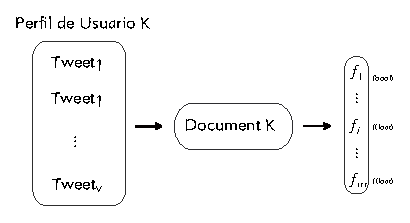
\includegraphics[width=.65\linewidth, , height=.2\textheight]{images/trepre.eps}
	 	\caption[Rasgos Manuales]{Representación de perfil mediante rasgos manuales}
	 	\label{trepre}
	 \end{figure}
	 
	 
	 